\documentclass[12pt]{article}
\usepackage[english]{babel}
\usepackage[utf8]{inputenc}

\usepackage{geometry}
\geometry{
	letterpaper, 
	portrait, 
	top=.75in,
	left=.8in,
	right=.75in,
	bottom=.5in		} 	% Page Margins
	
%% additional packages for nice things
\usepackage{amsmath} 	% for most math
\usepackage{commath} 	% for abs
\usepackage{lastpage}	% for page count
\usepackage{amssymb} 	% for therefore
\usepackage{graphicx} 	% for image handling
\usepackage{wrapfig} 	% wrap figures
\usepackage[none]{hyphenat} % for no hyphenations
\usepackage{booktabs} 	% enhanced table qualities
\usepackage{array} 		% for >{} column characterisctis
\usepackage{physics} 	% for easier derivative \dv....
\usepackage{tikz} 		% for graphic@!
\usepackage{circuitikz} % for circuits!
\usetikzlibrary{arrows.meta} % for loads
\usepackage[thicklines]{cancel}	% for cancels
\usepackage{xcolor}		% for color cancels
\usepackage[per-mode=fraction]{siunitx} % for si units and num
\usepackage{fancyhdr} 	% for header
\usepackage{comment}	% for ability to comment out large sections
\usepackage{multicol}	% for multiple columns using multicols
\usepackage[framed,numbered]{matlab-prettifier} % matlab sytle listing
\usepackage{marvosym} 	% for boltsymbol lightning
\usepackage{pdflscape} 	% for various landscape pages in portrait docs.
\usepackage{float}
\usepackage{fancyvrb}	% for Verbatim (a tab respecting verbatim)
\usepackage{enumitem}	% for [resume] functionality of enumerate
\usepackage{subfigure}

%% package config 
\sisetup{output-exponent-marker=\ensuremath{\mathrm{E}}} % for engineer E
\renewcommand{\CancelColor}{\color{red}}	% for color cancels
\lstset{aboveskip=2pt,belowskip=2pt} % for more compact table
\def\arraystretch{1.4} % adjust size of arrays
%\arraycolsep=1.4pt\def
\setlength{\parindent}{0cm} % Remove indentation from paragraphs
\setlength{\columnsep}{0.5cm}
\lstset{
	style      = Matlab-editor,
	basicstyle = \ttfamily\footnotesize, % if you want to use Courier - not really used?
}
\renewcommand*{\pd}[3][]{\ensuremath{\dfrac{\partial^{#1} #2}{\partial #3}}} % for larger pd fracs
\renewcommand{\real}[1]{\mathbb{R}\left\{ #1 \right\}}	% for REAL symbol
\newcommand{\imag}[1]{\mathbb{I}\left\{ #1 \right\}}	% for IMAG symbol
\definecolor{m}{rgb}{1,0,1}	% for MATLAB matching magenta
	
%% custom macros
\newcommand\numberthis{\addtocounter{equation}{1}\tag{\theequation}} % for simple \numberthis command
\newcommand{\equal}{=} % so circuitikz can have an = in the labels
\newcolumntype{L}[1]{>{\raggedright\let\newline\\\arraybackslash\hspace{0pt}}m{#1}}
\newcolumntype{C}[1]{>{\centering\let\newline\\\arraybackslash\hspace{0pt}}m{#1}}
\newcolumntype{R}[1]{>{\raggedleft\let\newline\\\arraybackslash\hspace{0pt}}m{#1}}

%% Header
\pagestyle{fancy} % for header stuffs
\fancyhf{}
\rhead{Thad Haines \\ Page \thepage\ of \pageref{LastPage}}
\chead{Initial Tgov1 Model Validation \\}
\lhead{Research \\ }
% spacing
\headheight 29 pt
\headsep 6 pt

\begin{document}
	\begin{figure}[ht!]
		\begin{center}
		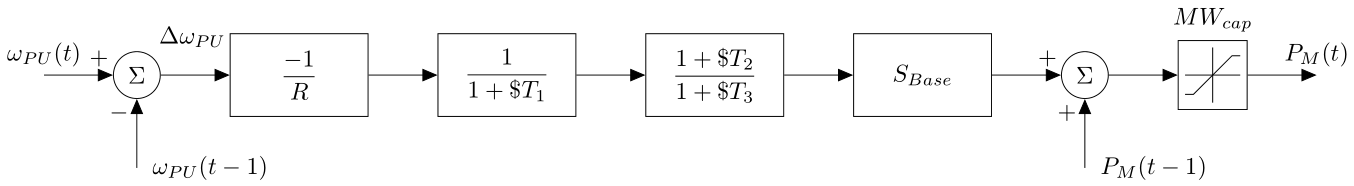
\includegraphics[width=\linewidth]{tgov1_model}\vspace{-1em}
		\caption{Tgov1 python Model}\vspace{1em}
		\label{tgov1}		 

		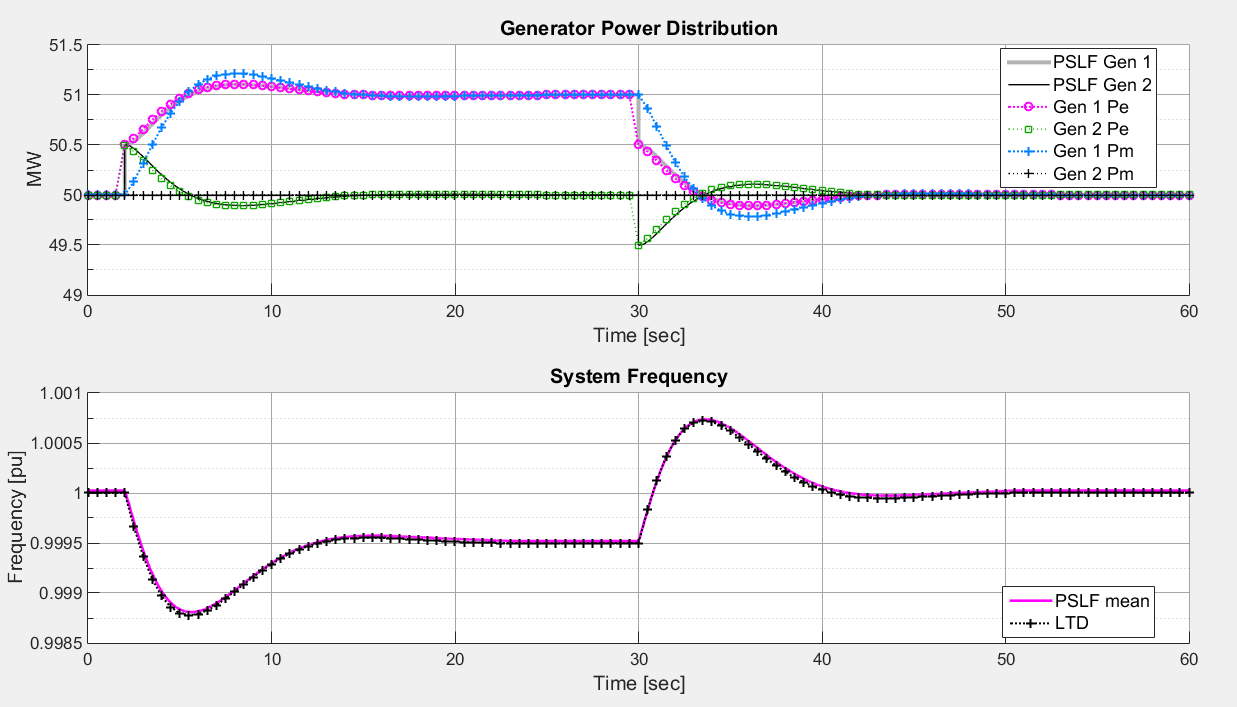
\includegraphics[width=.95\linewidth]{matlab_comparison03}  \vspace{-1em}
		\caption{Step Simulation Comparison - 0.5 second ts}\vspace{+.5em}
		\label{step1}
			
		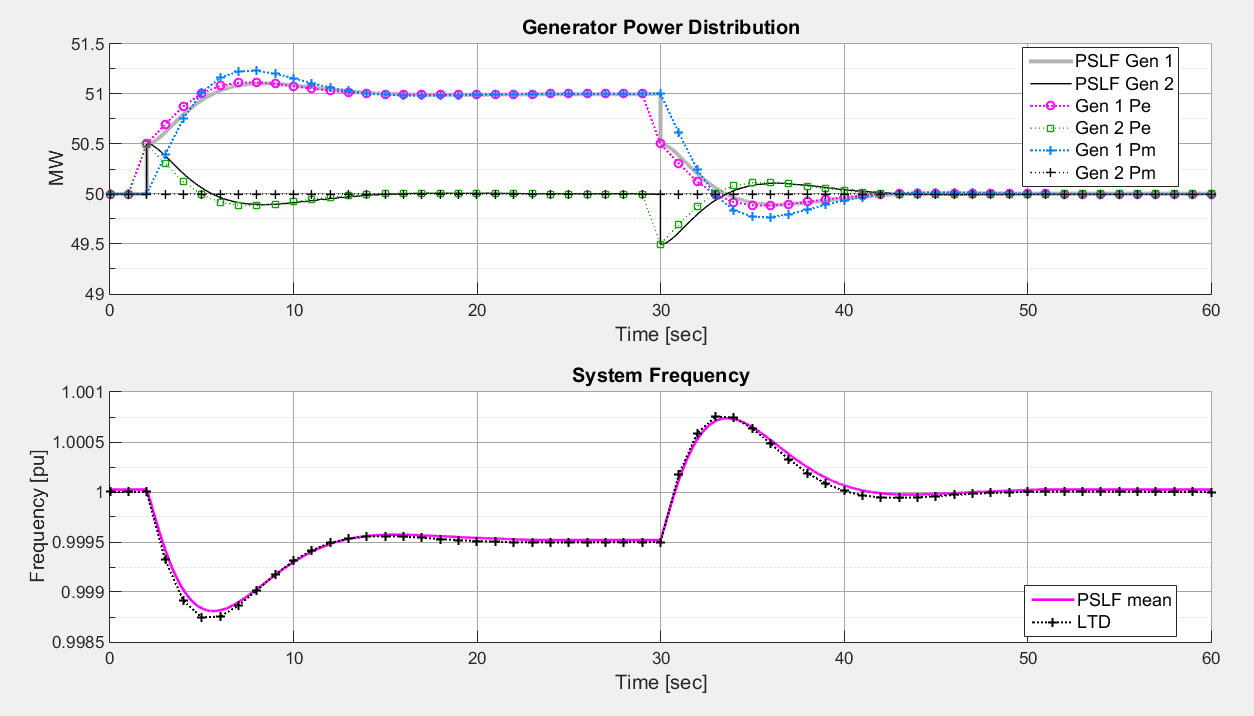
\includegraphics[width=.95\linewidth]{matlab_comparison04}  \vspace{-1em}
		\caption{Step Simulation Comparison - 1.0 second ts}
		\label{step2}
			\end{center}
		\end{figure}
\pagebreak
	\begin{figure}[ht!]
	\begin{center}

		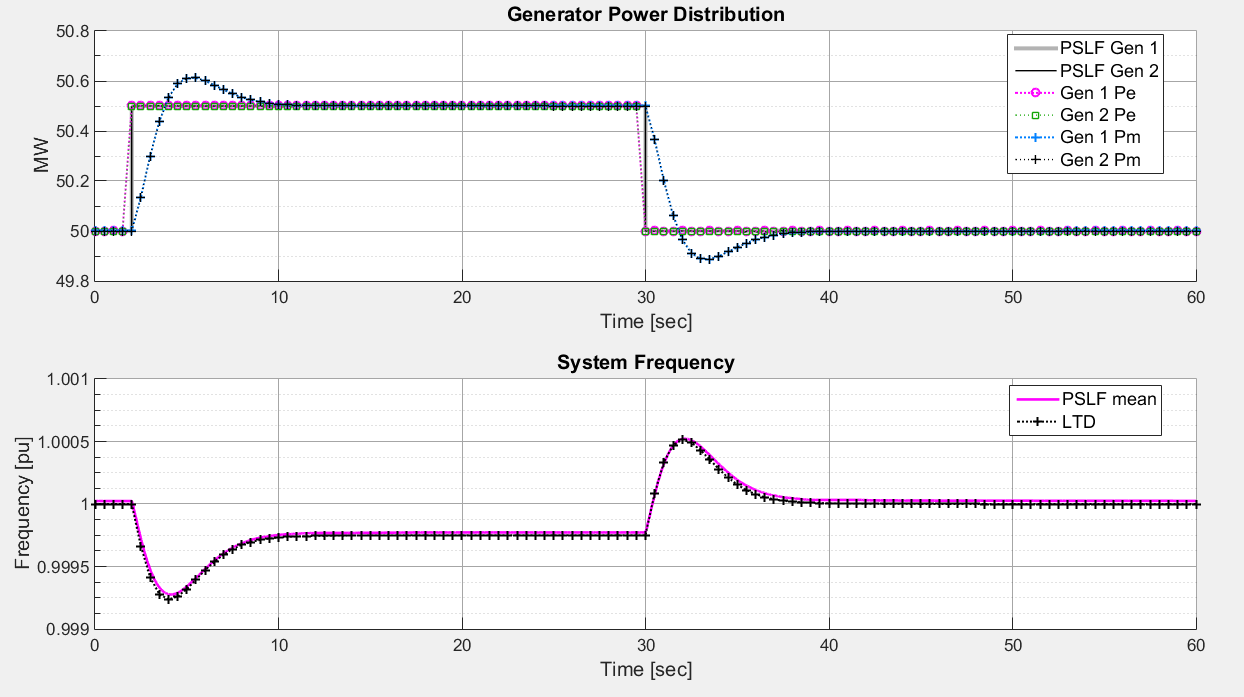
\includegraphics[width=.75\linewidth]{2gov_PSLF_comparison01}  \vspace{-1em}
		\caption{Step Simulation Comparison - Dual Governors - 0.5 second ts}
		\label{2gov1}\vspace{1em}
		
		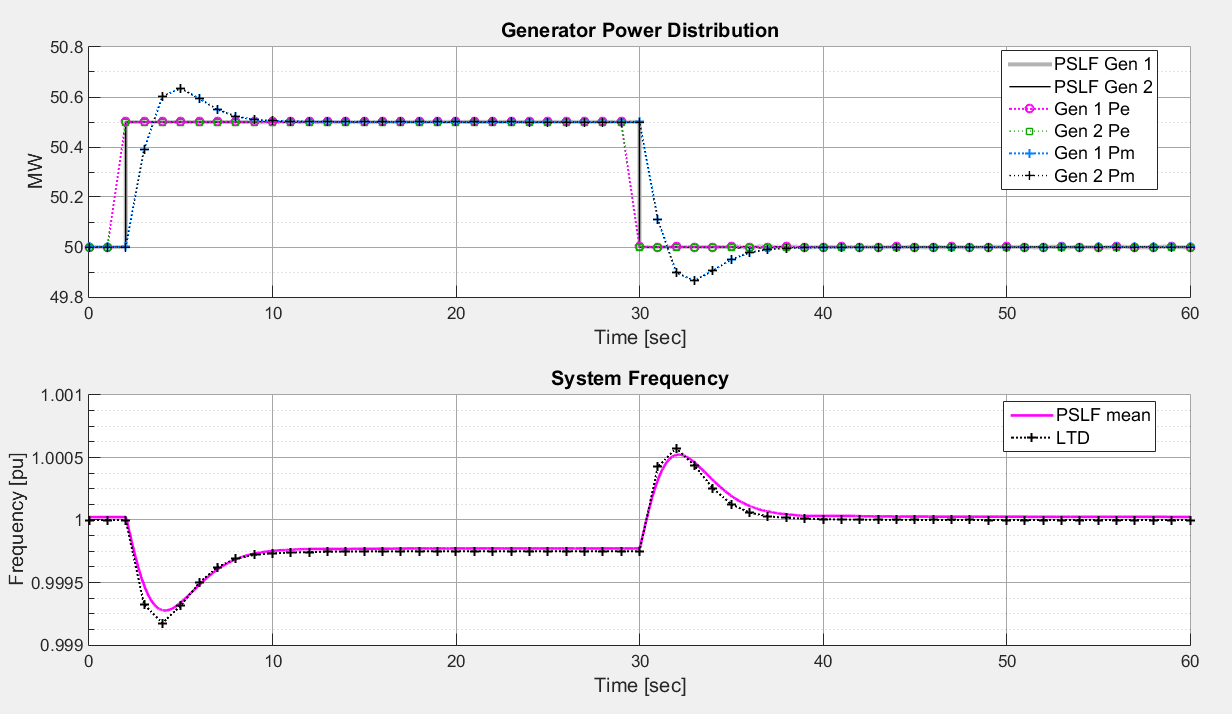
\includegraphics[width=.75\linewidth]{2gov_PSLF_comparison02}  \vspace{-1em}
		\caption{Step Simulation Comparison - Dual Governors - 1.0 second ts}
		\label{2gov2}\vspace{1em}
		
		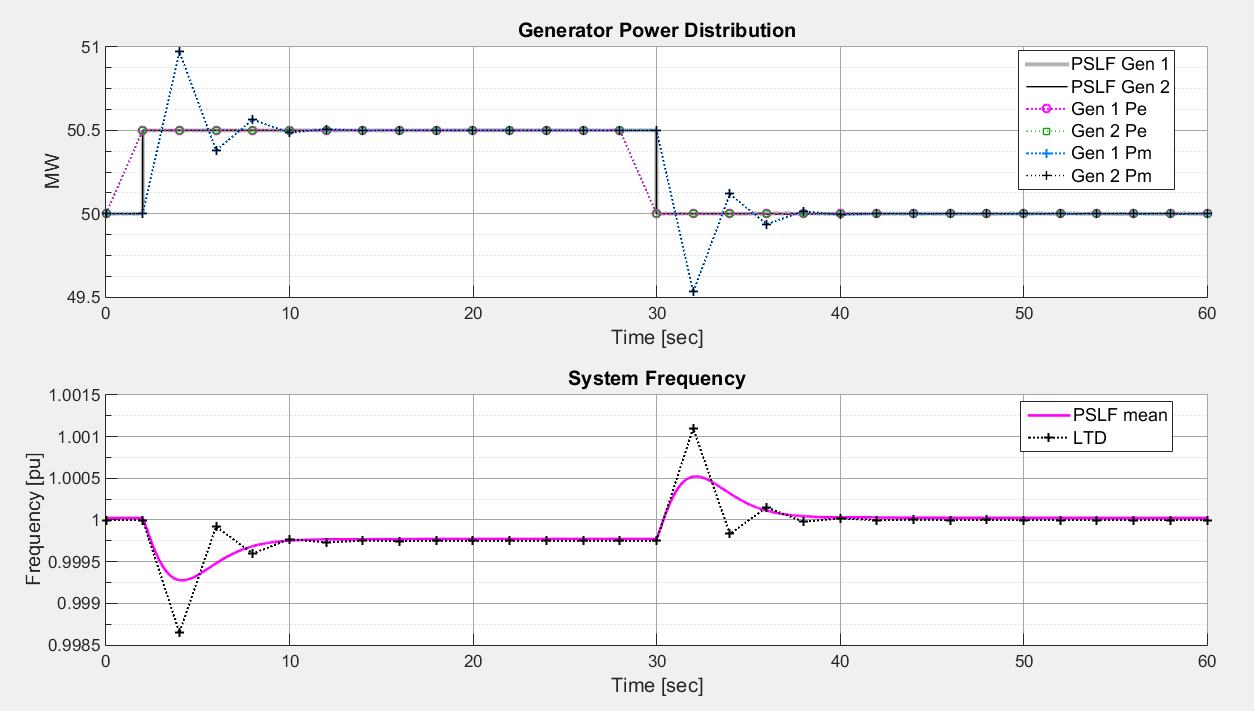
\includegraphics[width=.75\linewidth]{2gov_PSLF_comparison03}  \vspace{-1em}
		\caption{Step Simulation Comparison - Dual Governors - 2.0 second ts}
		\label{2gov3}\vspace{1em}
		
		%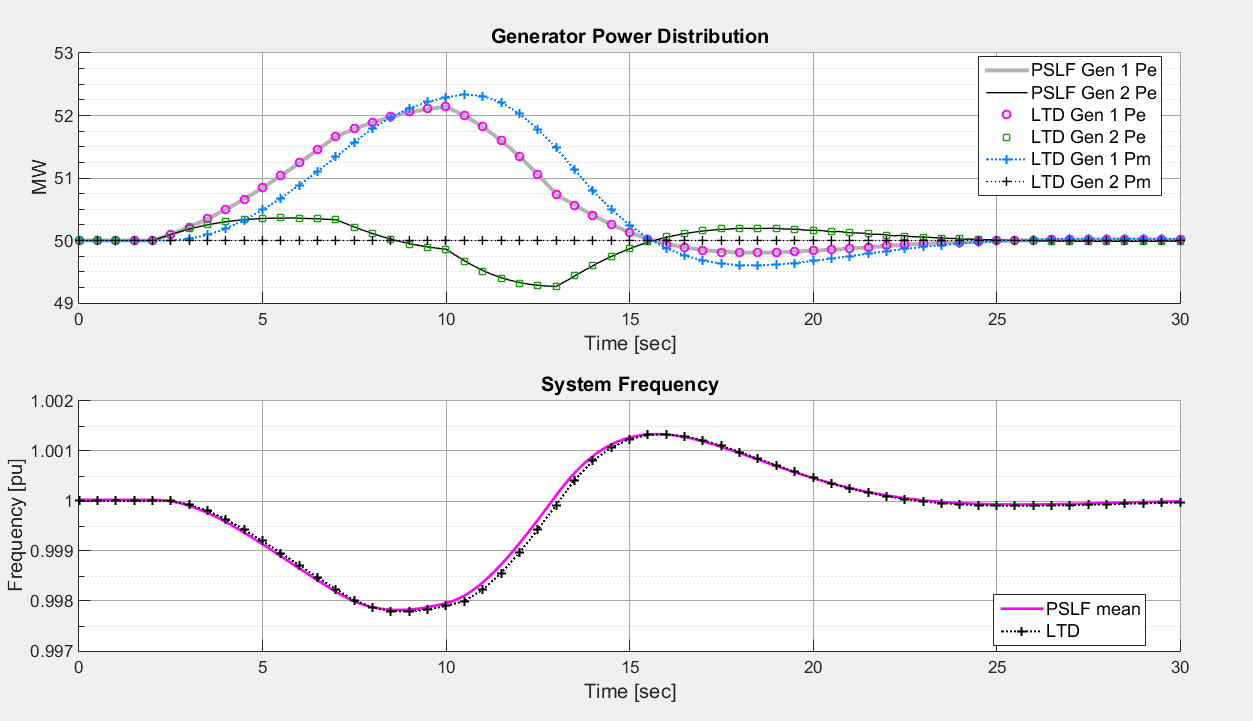
\includegraphics[width=.7\linewidth]{tgovWagent}\vspace{-1em}
		%\caption{Ramp Simulation Comparison - 0.5 second ts}
		%\label{ramp1}		 
		
	\end{center}
\end{figure}

\begin{comment}

Python Code:
\begin{lstlisting}[language=Python]
import numpy as np
import scipy.signal as sig
import matplotlib.pyplot as plt
import scipy.io as sio

# Inputs
Pref = .5 # will be a PU of Pref from Generator
delta_w = 0.0

# Simulation Parameters
t = np.linspace(0,30,101)
R = 0.05
Vmax = 1.0
Vmin = 0.0
T1 = 0.5
T2 = 3.0
T3 = 10.0
Dt = 0.0

# System Creations
sys1 = sig.TransferFunction(1,[T1, 1])
sys2 = sig.TransferFunction([T2, 1],[T3, 1])

# Input to system
u = (Pref-delta_w)/R

# First Block
_, y1, x1 = sig.lsim2(sys1, [u]*t.size, t)

# limit Valve position
for x in range(t.size):
    if y1[x]>Vmax:
        y1[x] = Vmax
    elif y1[x]<Vmin:
        y1[x] = Vmin

# Second block
_, y2, x2 = sig.lsim2(sys2, y1, t)

# Addition of damping
y2 = y2 + [delta_w*Dt]*y2.size

# Plot output
plt.plot(t,y2, label="Pmech Out")
plt.plot(t,[u*R]*t.size, label="Pref In")
plt.title('SciPy Simulated Tgov1')
plt.ylabel(r'$P_{mech}$ [PU]')
plt.xlabel('Time [sec]')
plt.grid()
plt.legend()
plt.show()

# Output data dictionary as .mat
pyTgov = {'t_py': t,
          'y_py': y2,}
sio.savemat('tgovTest', pyTgov)
\end{lstlisting}

\end{comment}

\end{document}
